\documentclass{article}
\usepackage[utf8]{inputenc}

% Page setup
\usepackage[a4paper,landscape,margin=2cm]{geometry}
\usepackage{amsmath}

% Typography
\usepackage[scaled]{helvet}
\let\familydefault\sfdefault

\usepackage[usenames,svgnames]{xcolor}
\usepackage{tikz,pgfplots}
\usetikzlibrary{positioning,arrows,intersections,calc}

\definecolor{colorfile}     {RGB}{ 79,142,209}
\definecolor{colorsummary}  {RGB}{143,232,186}
\definecolor{colortext}     {RGB}{ 29, 29, 27}

\begin{document}
\pagestyle{empty}
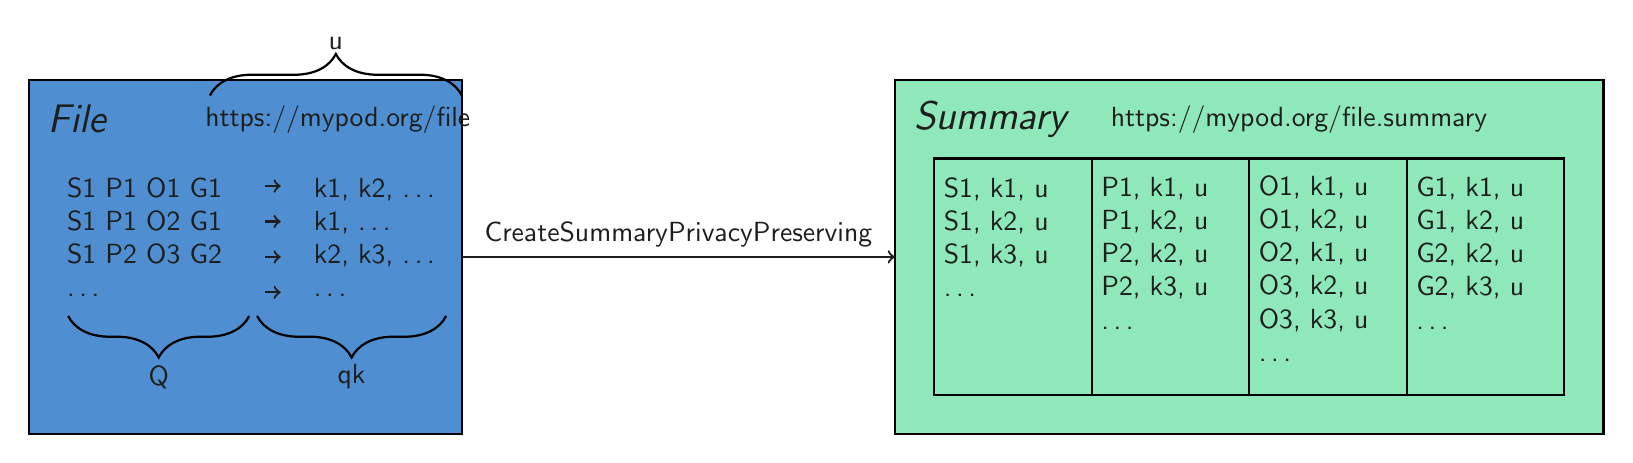
\begin{tikzpicture}[
    node distance = 10em, auto, thick,
    title/.style={text=colortext,font={\Large\itshape}},
    person/.style={text=colorwhite,font={\Large\bfseries}},
    code/.style={text=colortext,font={}},
    key/.style={text=colorkey,font={\tiny\itshape}}
]

    % File
    \draw[fill=colorfile] (0,4) rectangle (5.5,-0.5);
    \node[title,text width=10em] at (2,3.5) {File};
    \node[code,text width=10em] at (4,3.5) {https://mypod.org/file};
    \node[code,text width=20em] at (4,2) {S1 P1 O1 G1\\S1 P1 O2 G1\\S1 P2 O3 G2\\\ldots};
    
    % Keys
    \node[code,text width=5em] at (4.5,2) {k1, k2, \ldots\\k1, \ldots\\k2, k3, \ldots\\\ldots};
    \draw[->,thick,colortext] (3,2.65) -- (3.2,2.65);
    \draw[->,thick,colortext] (3,2.20) -- (3.2,2.20);
    \draw[->,thick,colortext] (3,1.75) -- (3.2,1.75);
    \draw[->,thick,colortext] (3,1.30) -- (3.2,1.30);
    
    % Braces
    \draw [decorate,decoration={brace,amplitude=15pt}] (2.3,3.8) -- (5.5,3.8) node [code,midway,yshift=13pt] {u};
    %\draw [decorate,decoration={brace,amplitude=15pt}] (0.5,1) -- (0.5,3) node [code,midway,xshift=-13pt] {Q}; % Q on left-hand side
    \draw [decorate,decoration={brace,amplitude=15pt,mirror}] (0.5,1) -- (2.8,1) node [code,midway,yshift=-30pt] {Q};
    \draw [decorate,decoration={brace,amplitude=15pt,mirror}] (2.9,1) -- (5.3,1) node [code,midway,yshift=-30pt] {qk};
    
    % Summary
    \draw[fill=colorsummary] (11,4) rectangle (20,-0.5);
    \node[title,text width=10em] at (13, 3.5) {Summary};
    \node[code,text width=10em] at (15.5,3.5) {https://mypod.org/file.summary};
    
    % Components
    \draw[fill=colorsummary] (11.5,3) rectangle (13.5,0);
    \node[code,text width=5em] at (12.5,2) {S1, k1, u\\S1, k2, u\\S1, k3, u\\\ldots};
    \draw[fill=colorsummary] (13.5,3) rectangle (15.5,0);
    \node[code,text width=5em] at (14.5,1.8) {P1, k1, u\\P1, k2, u\\P2, k2, u\\P2, k3, u\\\ldots};
    \draw[fill=colorsummary] (15.5,3) rectangle (17.5,0);
    \node[code,text width=5em] at (16.5,1.6) {O1, k1, u\\O1, k2, u\\O2, k1, u\\O3, k2, u\\O3, k3, u\\\ldots};
    \draw[fill=colorsummary] (17.5,3) rectangle (19.5,0);
    \node[code,text width=5em] at (18.5,1.8) {G1, k1, u\\G1, k2, u\\G2, k2, u\\G2, k3, u\\\ldots};

    % Arrows
    \draw[->,thick,colortext] (5.5,1.75) -- (11,1.75) node[midway] {CreateSummaryPrivacyPreserving};

\end{tikzpicture}
\end{document}
